\subsection{Frequenzantwort MIMO}
    Im MIMO Fall ist der Eingang $u(t)$ ein Vektor harmonischer Funktionen:
    \begin{equation*}
        u(t)=
        \begin{bmatrix}
        \mu_1\cdot\cos\left(\omega t + \varphi_1\right)\cdot h(t)\\
        \mu_2\cdot\cos\left(\omega t + \varphi_2\right)\cdot h(t)\\
        \dots\\
        \mu_m\cdot\cos\left(\omega t + \varphi_m\right)\cdot h(t)\\
        \end{bmatrix}
    \end{equation*}
    DieFrequenzanalyse beschränkt sich auf eine gemeinsame frei wählbare Anregungsfrequenz $\omega$ auf allen Kanälen. Die Anregungsmagnituden $\mu_i$ und -phasen $\varphi_i$ können separat gewählt werden. Laplace-Transformation von $u(t)$ führt zu:
    \begin{equation*}
        U(s)=
        \begin{bmatrix}
        e^{\varphi_1\cdot s/\omega} \cdot \mu_1 \cdot \frac{s}{s^2+\omega^2}\\
        e^{\varphi_2\cdot s/\omega} \cdot \mu_2 \cdot \frac{s}{s^2+\omega^2}\\
        \dots\\
        e^{\varphi_m\cdot s/\omega} \cdot \mu_m \cdot \frac{s}{s^2+\omega^2}\\
        \end{bmatrix}
        = e^{\Phi\cdot s/\omega}\cdot \mu\cdot\frac{s}{s^2+\omega^2}
    \end{equation*}
    mit $\Phi = \operatorname{diag}(\varphi_i)\in\mathbb{R}^{m\times m}$ und $\mu = [\mu_1,\dots,\mu_m]^\top \in\mathbb{R}^m$
    
    Damit ergibt sich für den Ausgang im eingeschwungenen Zustand:
    \begin{gather*}
        y_\infty(t) = 
        \begin{bmatrix}
            \nu_1\cdot\cos\left(\omega t +\psi_1\right)\\
            \nu_2\cdot\cos\left(\omega t +\psi_2\right)\\
            \dots\\
            \nu_m\cdot\cos\left(\omega t +\psi_m\right)
        \end{bmatrix}\\
        Y(s) = e^{\Psi\cdot s/\omega}\cdot\nu\cdot\frac{s}{s^2+\omega^2}
    \end{gather*}
     mit $\Psi = \operatorname{diag}(\psi_i)\in\mathbb{R}^{m\times m}$ und $\nu = [\nu_1,\dots,\nu_m]^\top \in\mathbb{R}^m$
     
     Da für $Y(\jw) = P(\jw)\cdot U(\jw)$ gilt ergibt sich:
     \begin{gather*}
        e^{\Psi}\cdot\nu = P(\jw) \cdot e^{\Phi}\cdot \mu\\
        \underbrace{y}_{e^{\Psi}\cdot\nu} = \underbrace{M}_{P(\jw)} \cdot \underbrace{u}_{e^{\Phi}\cdot \mu}
     \end{gather*}
     Wir stellen fest, dass der Ausgang $y$ eine lineare Abbildung von $u$ ist. Es gilt daher:
     \begin{equation*}
        \sigma_\textnormal{min}\big(P(\jw)\big) \leq \frac{\|\nu\|}{\|\mu\|} \leq \sigma_\textnormal{max}\big(P(\jw)\big)
     \end{equation*}
     Die Singulärwerte geben für den eingeschwungenen Zustand Schranken für den Betrag der Amplituden $\|\nu\|$. Sie sind ein Mass für den worst-case Amplitue die man bei der Anregung einer gegebenen Frequenz $\omega$ erwarten kann.
    
    \subsubsection{Bsp}
        Wir wollen das System
        \begin{equation*}
            P(s) = 
            \begin{bmatrix}
                \frac{1}{s^2+0.3s+1} &  \frac{0.2}{s^2+0.5s+1}\\
                \frac{0.2}{s^2+s+1} &   \frac{1}{s^2+s+1}
            \end{bmatrix}
        \end{equation*}
        für $\{\mu \,|\, \|\mu\|=1\}$ bei $\omega = 0.7$ rad/s so anregen, dass $\|\nu\| = \sigma_\textnormal{max}\big(P(j\cdot0.7)\big)$ gilt.
        
        \begin{figure}[H]
            \centering
            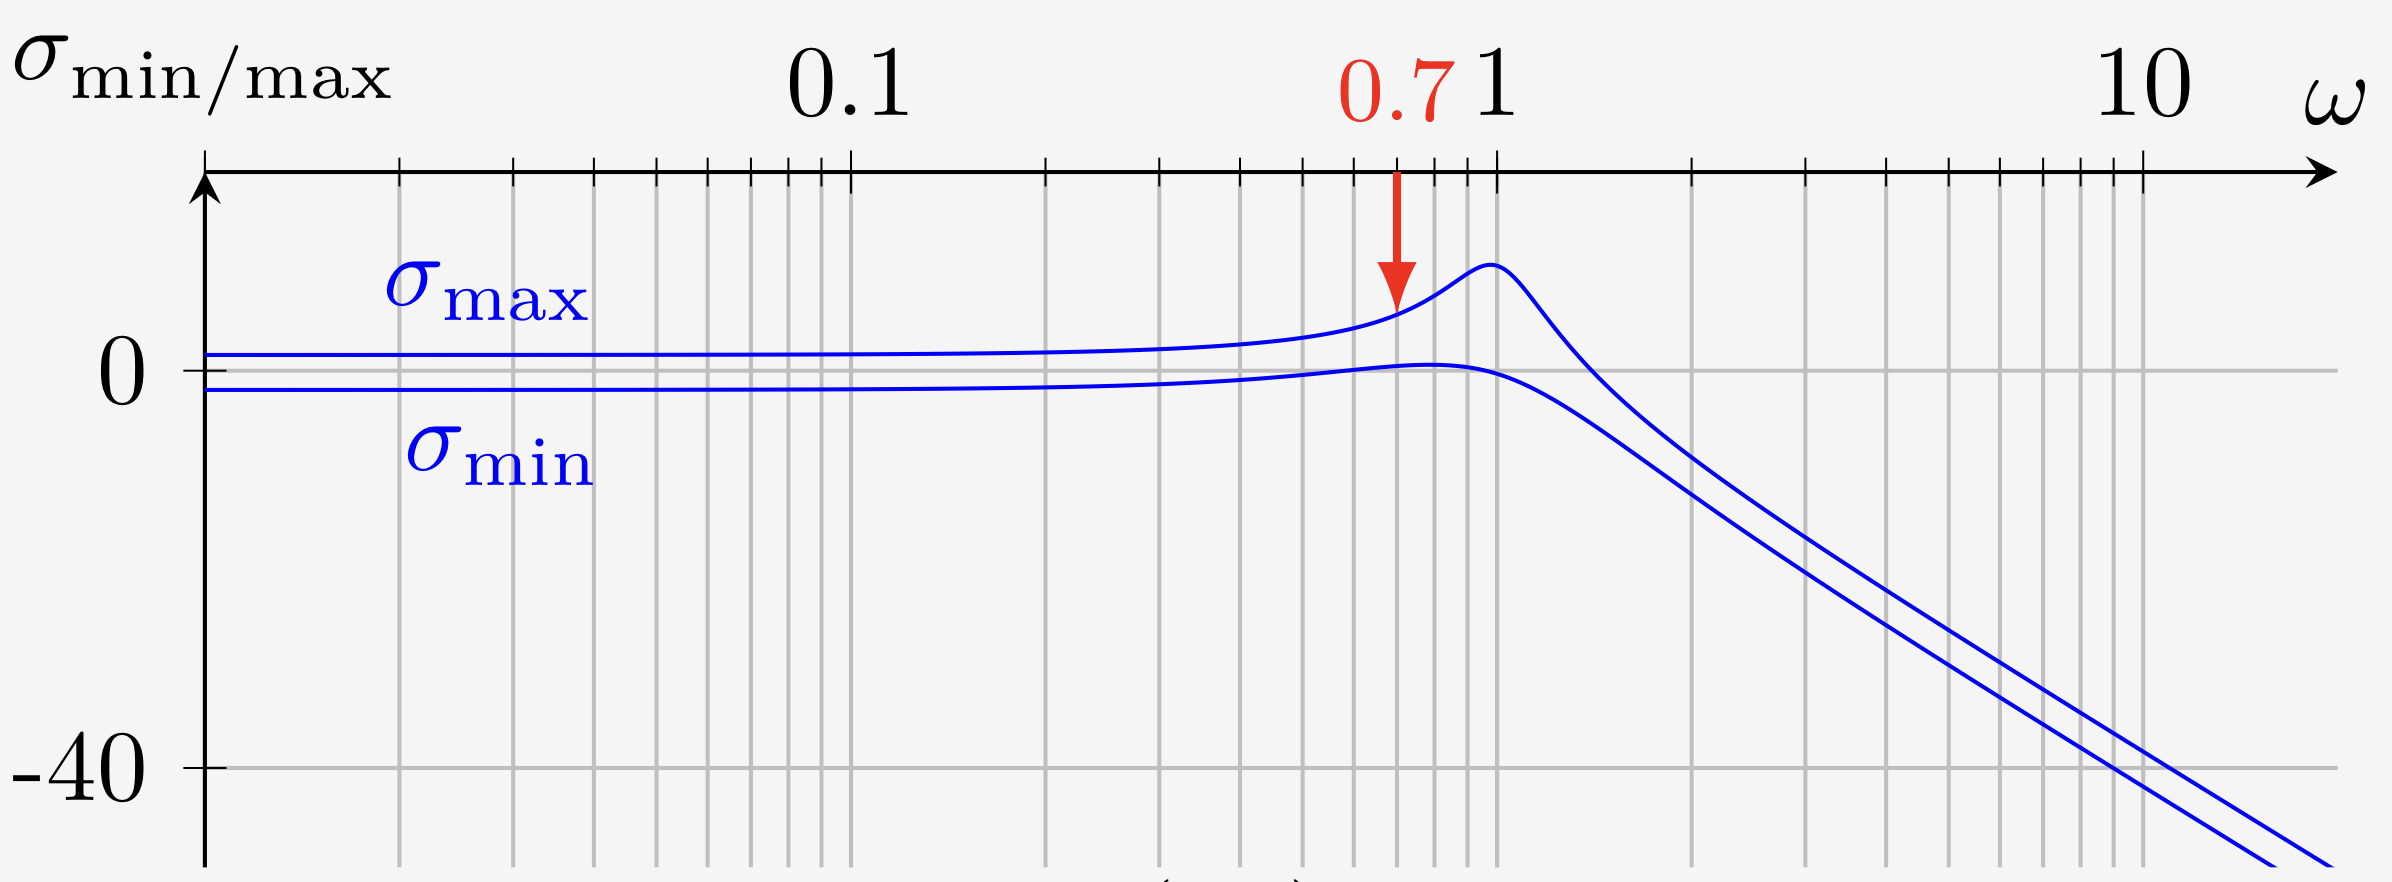
\includegraphics[width = 0.5\linewidth]{images/07/singular_val_plot.jpeg}
        \end{figure}
        
        Wir stellen fest, dass $\sigma_\textnormal{max}\big(P(j\cdot0.7)\big) = 1.914$. Die Ausgänge $y_1$ und $y_2$ werden je Amplituden $\nu_1$ und $\nu_2$ haben, die kleiner als 1.914 sind. Bei der maximalen Anregung wird die Norm  jedoch $\|\nu\| = 1.914$ sein.
        
        Um die Anregungsrichtung zu finden, bei der $\|\nu\|$ maxial wird, verwendet man die Singulärwertzerlegung der Matrix $P(j\cdot0.7)$:
        \begin{align*}
            P(j\cdot0.7) &= U\cdot\Sigma\cdot V^\top = \\ 
           &\begin{bmatrix}
           \textcolor{red}{-0.8724+0.3635j}  &   0.3089-0.1068j\\
           \textcolor{red}{-0.2167+0.2247j}  &   -0.6691+0.6675j
           \end{bmatrix}
           \cdot
           &\begin{bmatrix}
           \textcolor{blue}{1.914}    &   0\\
           0        &   1.056
           \end{bmatrix}
           \cdot\\
           &\begin{bmatrix}
           \textcolor{cyan}{-0.9344}  &   \textcolor{cyan}{-0.3525+0.0515j}\\
           0.3562   &   -0.9246+0.1351j
           \end{bmatrix}
        \end{align*}
        \textcolor{red}{Ausgangsrichtung der Maximalen Verstärkung} entspricht der ersten Spalte von $U$, die \textcolor{blue}{Maximale Verstärkung} entspricht dem höchsten Singulärwert, welcher an erster Stelle steht und die \textcolor{cyan}{Eingangsrichtung der maximalen Verstärkung} entspricht der ersten Zeile von $V^\top$. \big(MATLAB: \texttt{V(:,1)\big)}
        
        Die Maximale Richtung ist somit:
        \begin{gather*}
            \zeta_\textnormal{max} = 
            \begin{bmatrix}
            -0.9344\\ -0.3525+0.0515j
            \end{bmatrix}
            =
            \begin{bmatrix}
            e^{j\pi} & 0\\
            0 & e^{j2.9965}
            \end{bmatrix}
            \cdot
            \begin{bmatrix}
            0.9344\\ 0.3562
            \end{bmatrix}\\
            \Rightarrow u(t) = 
            \begin{bmatrix}
            0.9344\cdot\cos\left(0.7\cdot t + \pi\right)\\
            0.3562\cdot\cos\left(0.7\cdot t + 2.9965\right)
            \end{bmatrix}
        \end{gather*}
        
        \begin{figure}[H]
            \centering
            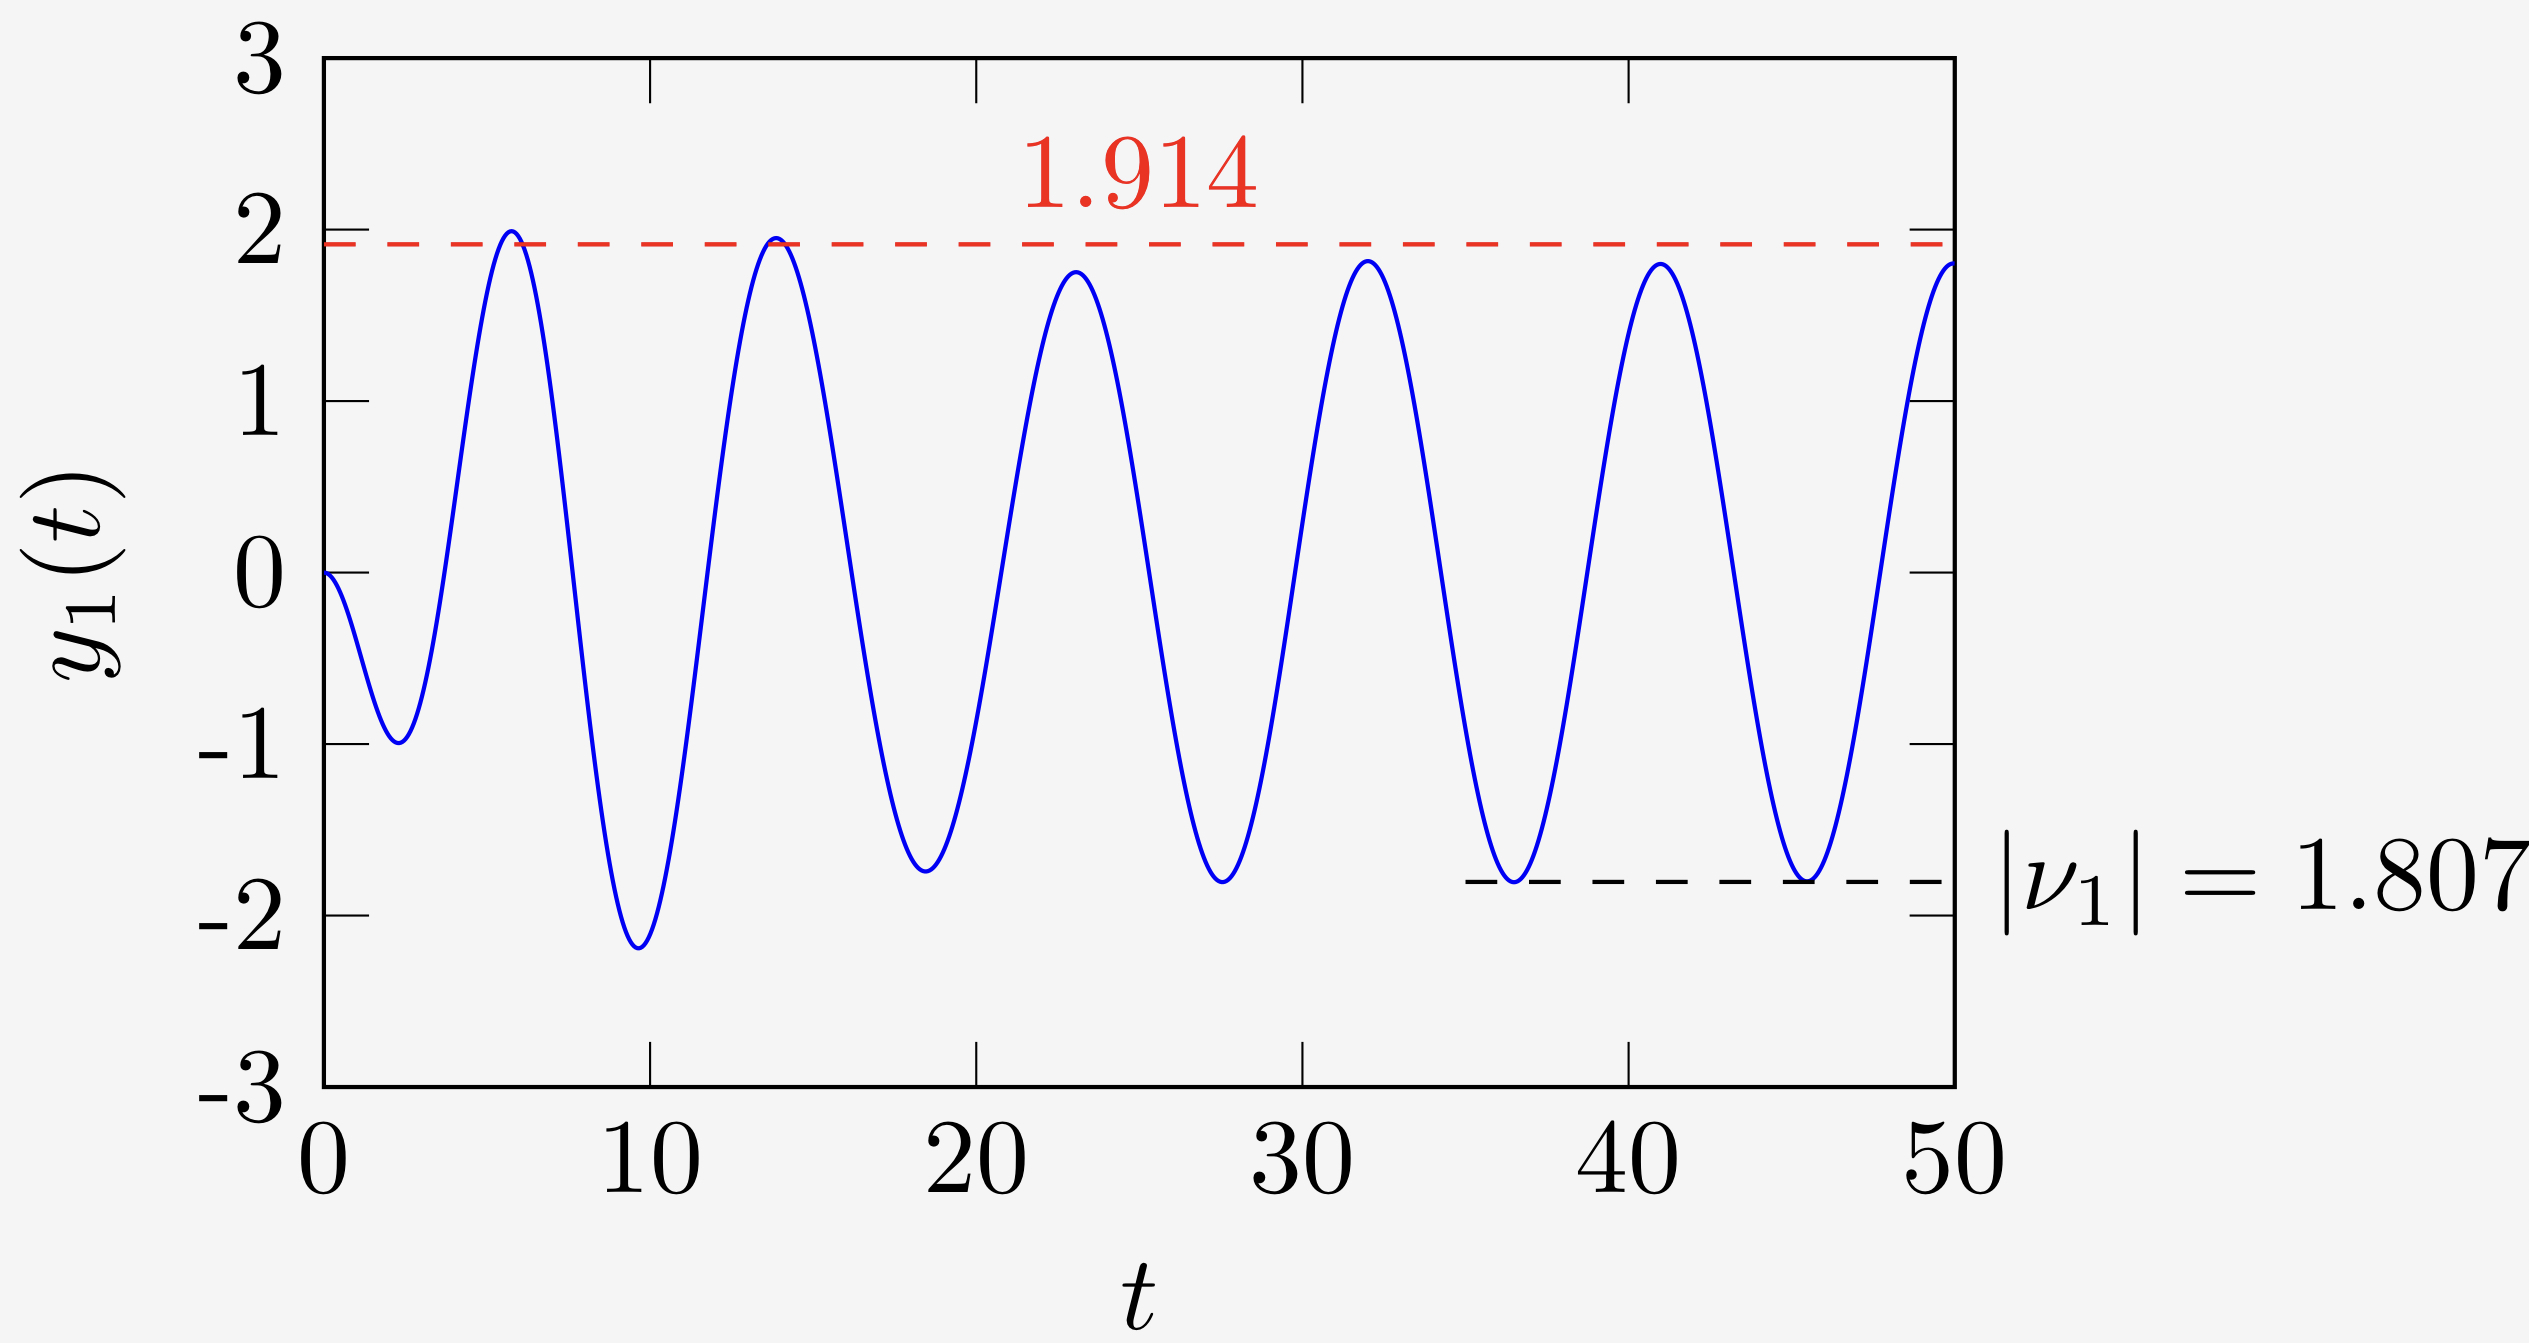
\includegraphics[width = 0.4\linewidth]{images/07/freq_resp_bsp_1.jpeg}
            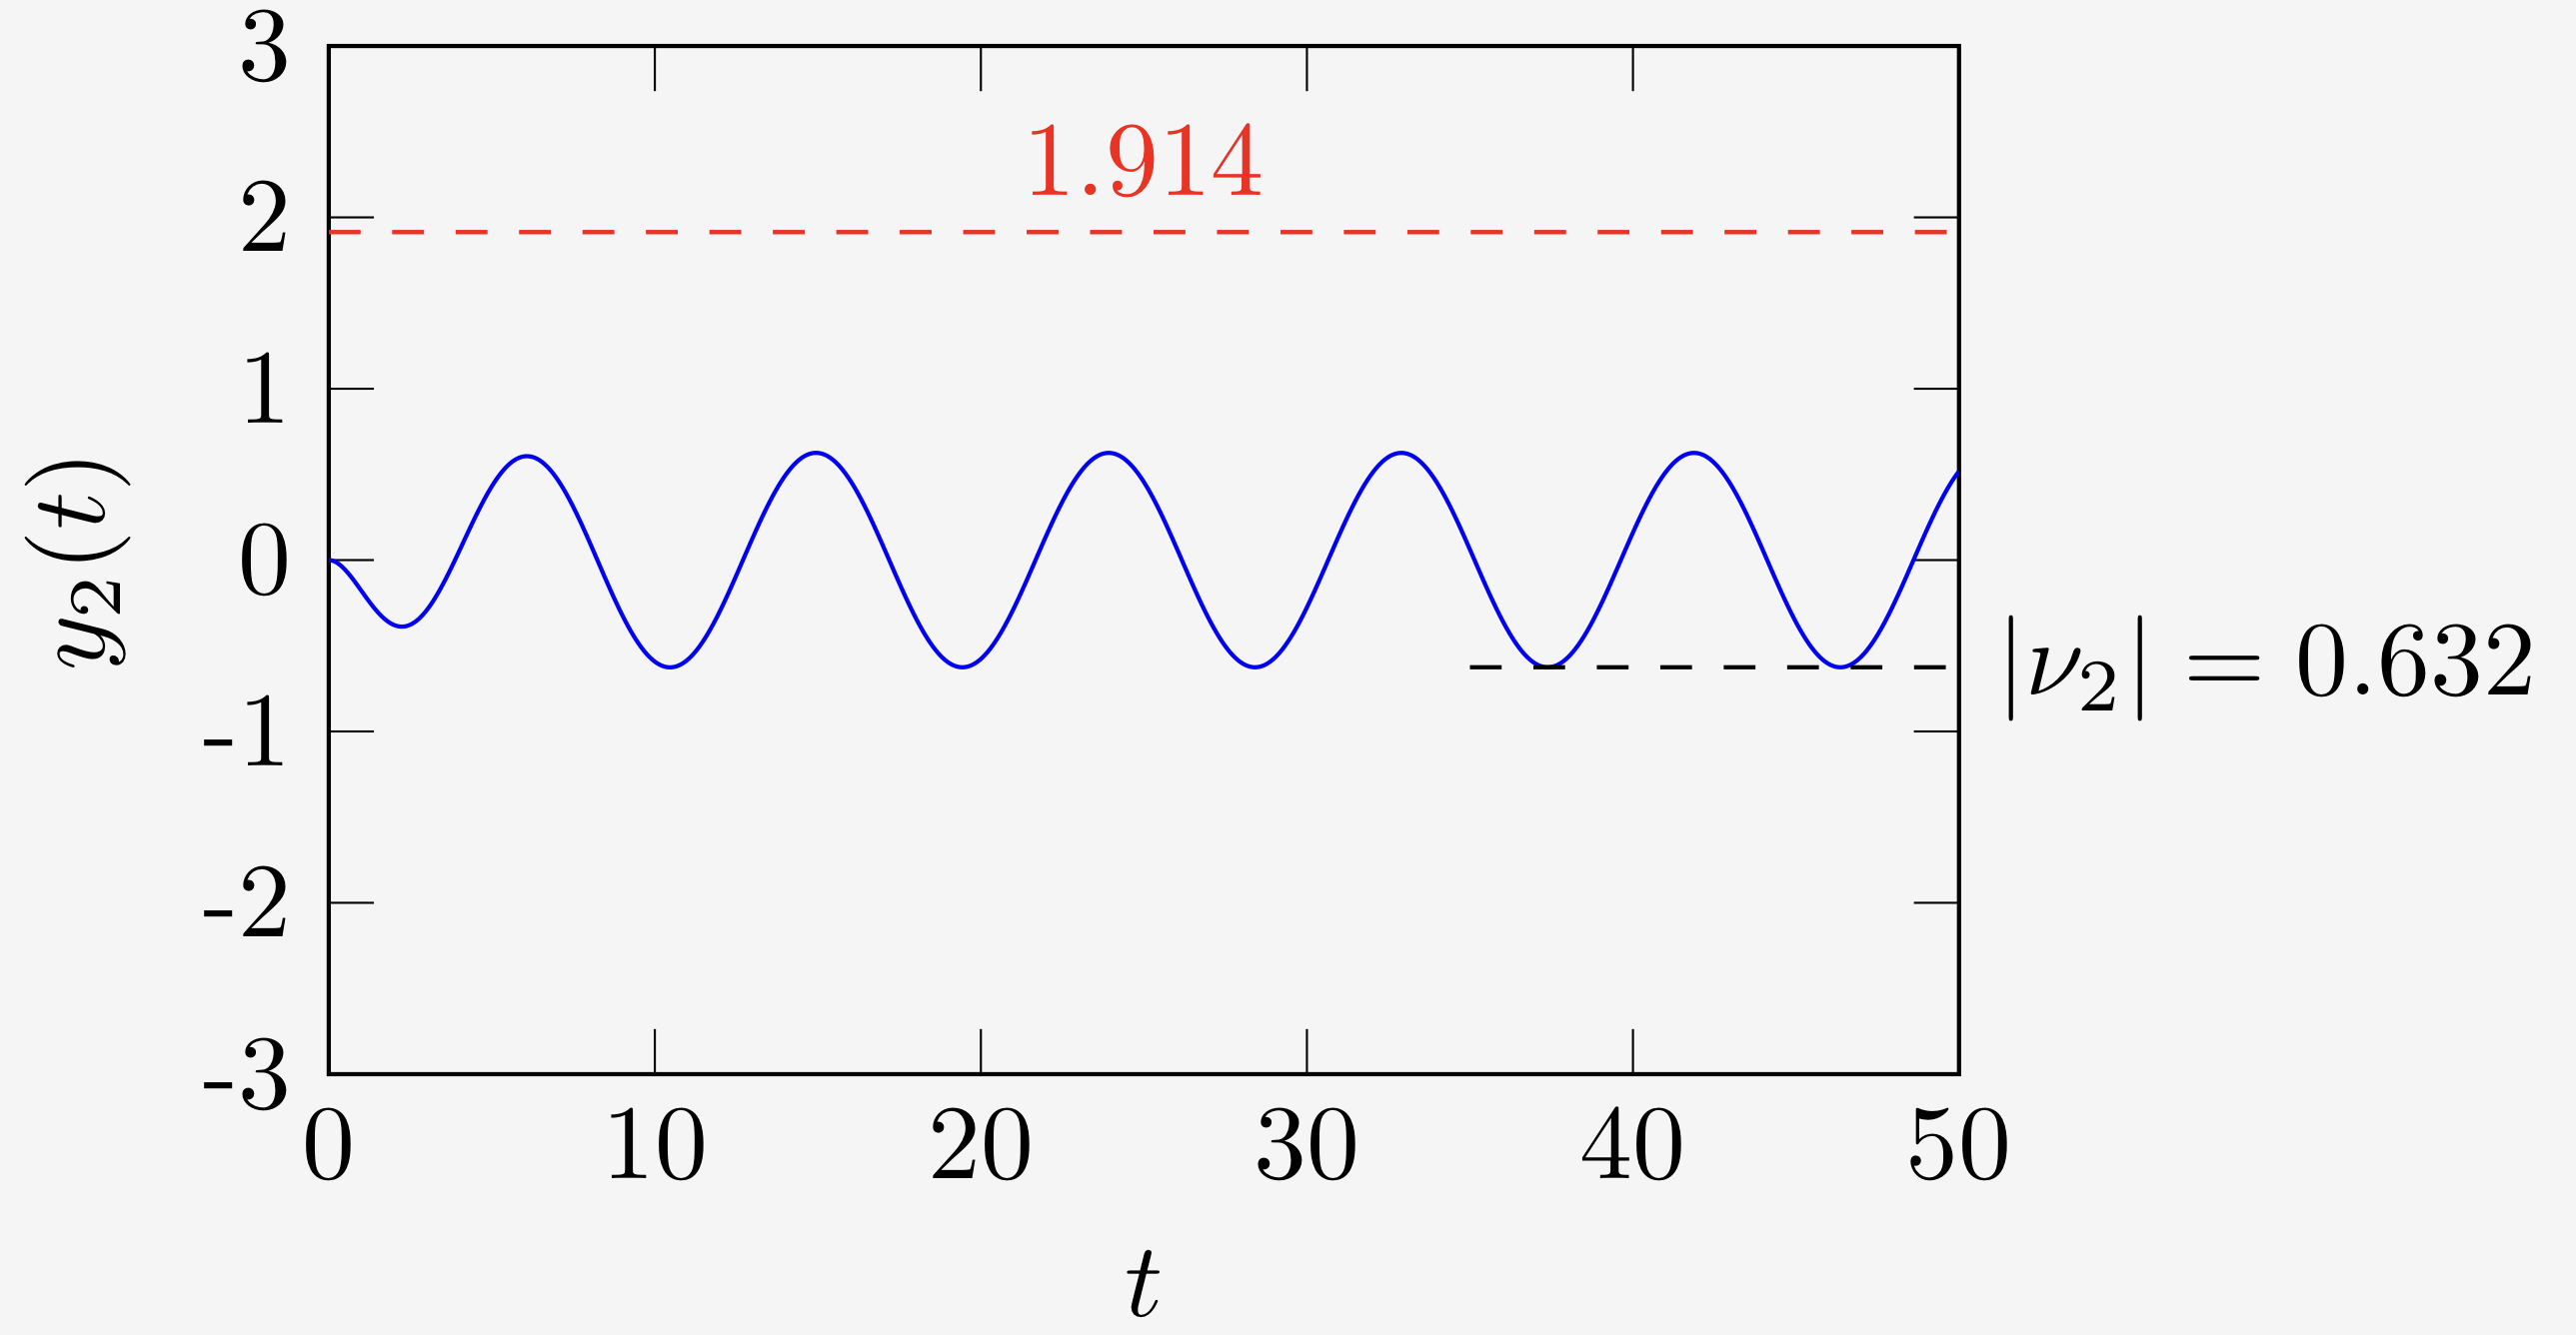
\includegraphics[width = 0.4\linewidth]{images/07/freq_resp_bsp_2.jpeg}
            \caption{Simulation des Systems mit Eingangssignal der Maximalen Verstärkung}
        \end{figure}
        
        \textbf{Bemerkungen:}
        \begin{itemize}
            \item \textbf{ACHTUNG} Beim Eingangssignal $T$ ablesen und $\omega = 2\pi/T$
            \item $|\nu_1| < \sigma_\textnormal{max} \quad\Rightarrow\quad y_{1,\infty} < \sigma_\textnormal{max}$
            \item $|\nu_2| < \sigma_\textnormal{max} \quad\Rightarrow\quad y_{2,\infty} < \sigma_\textnormal{max}$
            \item $\|\nu\|=\sigma_{\textnormal{max}}\cdot\underbrace{\|\mu\|}_{=1}$
            \item $\max(\|y(t)\|) < \|\nu\|$, da der Ausgang nicht unbedingt in Phase schwingt
            \item $\sqrt{|\nu_1|^2 + |\nu_2|^2} = 1.914 = \sigma_\textnormal{max}$ (Da maximale Richtung angeregt)
        \end{itemize}